\documentclass[conference]{IEEEtran}
\IEEEoverridecommandlockouts
% The preceding line is only needed to identify funding in the first footnote. If that is unneeded, please comment it out.
\usepackage{cite}
\usepackage{amsmath,amssymb,amsfonts}
\usepackage{algorithmic}
\usepackage{graphicx}
\usepackage{textcomp}
\usepackage{xcolor}
\usepackage{url}
\usepackage{float}
\def\BibTeX{{\rm B\kern-.05em{\sc i\kern-.025em b}\kern-.08em
    T\kern-.1667em\lower.7ex\hbox{E}\kern-.125emX}}

\begin{document}

\title{Practical Work I - Report\\
{\footnotesize \textsuperscript{}This report has been carried out for the ANADI Curricular Unit}
}

\author{
\IEEEauthorblockN{1\textsuperscript{st} Mariana Lages}
\IEEEauthorblockA{\textit{Instituto Politécnico do Porto} \\
\textit{ISEP - DEI}\\
Porto, Portugal \\
1200902@isep.ipp.pt}
\and

\IEEEauthorblockN{2\textsuperscript{nd}  Miguel Jordão}
\IEEEauthorblockA{\textit{Instituto Politécnico do Porto} \\
\textit{ISEP - DEI}\\
Porto, Portugal \\
1201487@isep.ipp.pt}
\and

\IEEEauthorblockN{3\textsuperscript{rd} Francisco Redol}
\IEEEauthorblockA{\textit{Instituto Politécnico do Porto} \\
\textit{ISEP - DEI}\\
Porto, Portugal \\
1201239@isep.ipp.pt}
}

\maketitle

\begin{abstract}
On this report, we utilized R language features to support our affirmations and conclusions.
Themes such data analysis, data modeling and non/parametric tests were used on the data from imported .csv files. 
\end{abstract}

\begin{IEEEkeywords}
regression, data analysis, data modeling, R language
\end{IEEEkeywords}

\section{Introduction}

Exploratory analysis is elected as the first step in a data analysis process, providing insights into a data set's characteristics. By exploring and summarizing data through numerous statistical and graphical procedures, 
researchers can identify patterns, anomalies, and potential outliers, which can guide further analysis and hypothesis testing, along with formulating theories around a certain subject.
In this research, we will discuss key statistical aspects of that character, such as exploratory analysis, parametric and non-parametric tests, linear regression, and data modelling based on the provided data sets.
By giving an insight into these techniques and their applications, we aim to emphasise the importance of these backbone concepts while doing scientific research.
In the proposed assignment, there are three distinct data sets which will be thoroughly described, along with the steps to dissect these.

\subsection{Pump Data set - Data Treatment}
The "DADOS1.csv" data set contains data about three electric submersible pumps (ESP) used to transport fluids in deep wells in oil extraction. The measurements in the provided data set were performed throughout one year (from June 1, 2013, to June 12, 2014).

The objective of this study is to optimize the company's production, through the analysis of the performance of the electric pumps.

Through several exploratory analysis methods, it becomes possible to find information hidden from the naked eye, which may enhance the understanding of the context in question, such as, for instance, comparing performance between the pumps.

\section{Exploratory Analysis - Pumps}
Before any calculation, we imported the data from the provided CSV file.

The first paragraph of this exercise consisted of adding a column to the data imported with the time in the POSIXct system and in a specific format ("yy/mm/dd HH:MM:SS GMT"). To do so, it was only necessary to convert the column of seconds already provided into dates.\\

The second paragraph asked for a graph to compare the engine temperature of the three pumps on the 4th of August 2013.

For this, the most suitable graph is a line graph, as it allows to clearly visualize the changes in engine temperature over time and easily compare the three pumps in a single graph. In addition, it is possible to identify trends, patterns and anomalies in the temperature values.

The graph obtained was as follows:

\begin{figure}[htbp]
    \centering{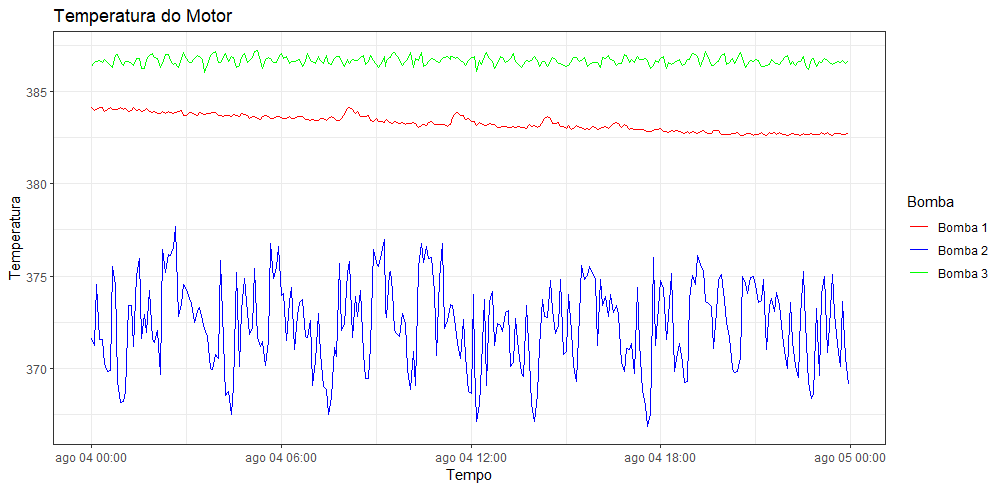
\includegraphics[width=9cm]{images/pumps/lineGraphMotorTemperature.png}}
    \caption{Line graph of motor temperature variation for each pump on August 4, 2013.}
    \label{pump_lineGraph_motorTemperature}
\end{figure}

Based on the analysis of the graph, it is possible to observe that pump 3 presents the highest values of motor temperature, while pump 2 has the lowest values. However, compared to the other pumps, pump 2 has the highest variation in values, oscillating between approximately 360 and 380.

In relation to pumps 1 and 3, the first one proves to be the pump with the lowest temperature variation, with values around 383 K and the third also does not show a large variation in its values, which are around 387 K.\\

The third paragraph consisted of making a box plot with the data from the previous paragraph and commenting on the results obtained.

The box plot is a useful graphical tool for analyzing the location and dispersion of data in a data set. In addition, it is possible to identify observations that are outside the data pattern, also known as outliers.

The box plot obtained was as follows:

\begin{figure}[H]
    \centering{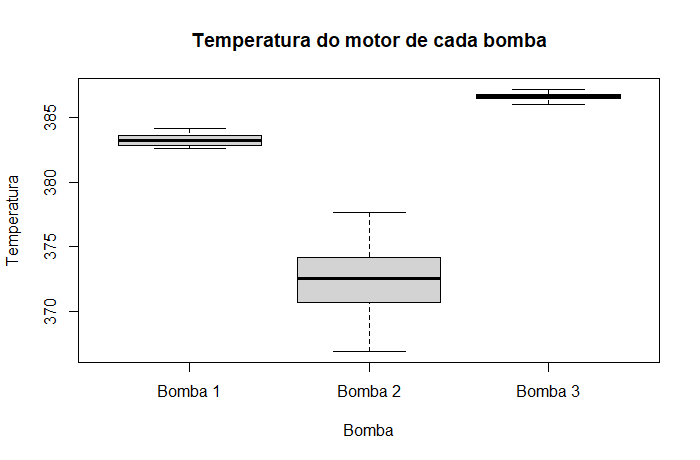
\includegraphics[width=9cm]{images/pumps/boxplotMotorTemperature.png}}
    \caption{Box plot of motor temperature variation for each pump on August 4, 2013.}
    \label{pump_boxplot_motorTemperature}
\end{figure}

Analyzing the results obtained, we can observe that the motor temperatures of pumps 1 and 3 are higher than those of pump 2. 

The median (represented by the darker line inside the boxes) of the motor temperature of pump 2 is around 373 K, while the medians for bombs 1 and 3 are approximately 383 and 386 K, respectively.

Another relevant factor to highlight is the distance between the minimum and maximum values of each pump, which indicates the data dispersion. In pump 2, there is a large spread of data, while in pumps 1 and 3, the spread is smaller.

Furthermore, the box (interquartile range - IQR) of pump 2 is larger than that of the other pumps, which indicates a higher frequency in the data distribution.\\

The fourth and last paragraph is divided into five other sub-paragraphs and states the following: "One way to assess the number of barrels produced in a day is to calculate the average of the oil rate measurements made on the day in question".

Taking this information into account, the first subparagraph consisted of creating a bar chart to compare the barrels of oil produced daily by pumps 1 and 2 in March 2014.

The bar chart obtained was as follows:

\begin{figure}[H]
    \centering{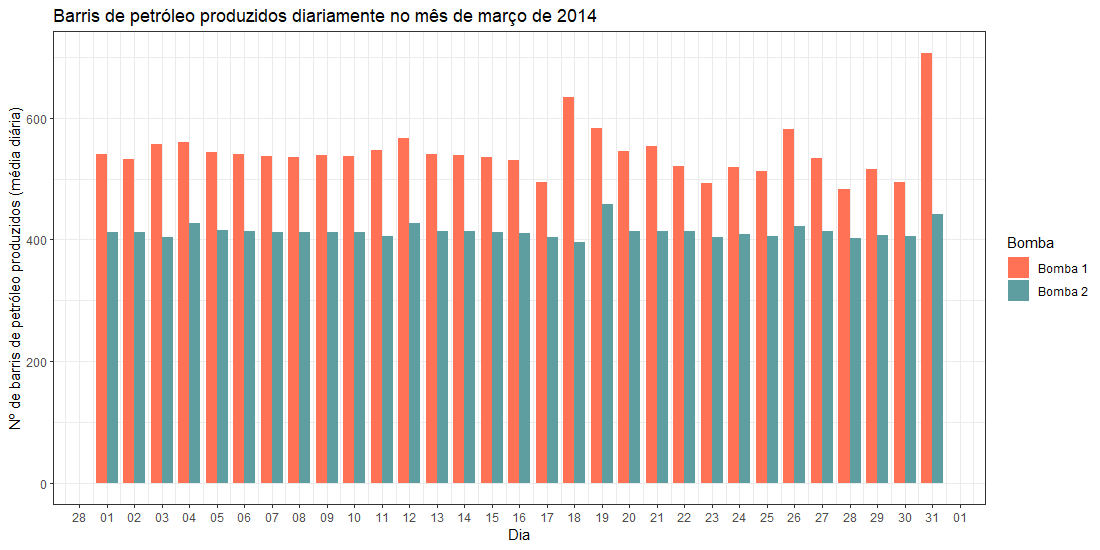
\includegraphics[width=9cm]{images/pumps/barGraphDailyProduction.png}}
    \caption{Bar chart of daily production of barrels of oil by pumps 1 and 2 in March 2014.}
    \label{pump_barChart_dailyProduction}
\end{figure}

By analyzing the bar chart, we can see that pump 1 surpassed pump 2 in the number of barrels of oil produced in all days of March 2014. 

The day with the highest number of barrels produced by pump 1 was the 31st, with a total of approximately 550 barrels, while pump 2 had its highest production on the 19th, with around 440 barrels. 

These results highlight the remarkable efficiency of pump 1 when compared with pump 2.\\

The second subparagraph required the identification of the month in which pump 1 obtained the highest extraction of barrels of oil, within the period between June 1, 2013, and May 31, 2014.

To answer the question, the approach adopted consisted of adding up the daily production of barrels of oil for each month in the referred period and then determining the month with the highest extraction of barrels by pump 1.

The table obtained was as follows:

\begin{figure}[H]
    \centering{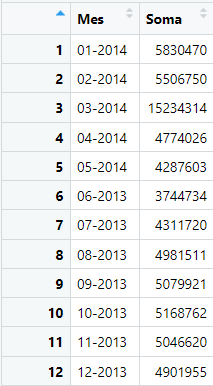
\includegraphics[width=4cm]{images/pumps/tableMonthlySums.png}}
    \caption{Table of the monthly sums of barrels of oil extracted by pump 1 between June 1, 2013, and May 31, 2014.}
    \label{pump_table_monthlySums}
\end{figure}

After analyzing the table, we can conclude that the month in which pump 1 extracted more barrels of oil was March 2014, as it is the month with the highest sum value.\\

In the third subparagraph, we were given a random sample of days between the previous dates (June 1, 2013, and May 31, 2014), in which the days were numbered in ascending order, with day 1 corresponding to June 1, 2013, and so on until the last day of the period, represented by the number corresponding to day 365.

From this sample, it is requested to calculate the daily production of pumps 1 and 2 on the selected days and the creation of a box plot to represent the obtained data.

The first step in analyzing the random sample of days is to convert the list of day numbers into their respective dates. The resulting list of dates is as follows: 2013-08-17, 2014-05-28, 2013-08-05, 2013-11-03, 2014-03-04, 2013-07-11, 2014-05-05, 2013-11-16, 2014-02-27 and 2014-02-23.

Now that we have the corresponding dates, the next step is to calculate the daily average for each pump in each of the days obtained and perform the box plot from these data.

When formulating the table with the data, one of the sample dates does not appear because there are no corresponding records in the original CSV data file for that date.

The box plot obtained was as follows:

\begin{figure}[H]
    \centering{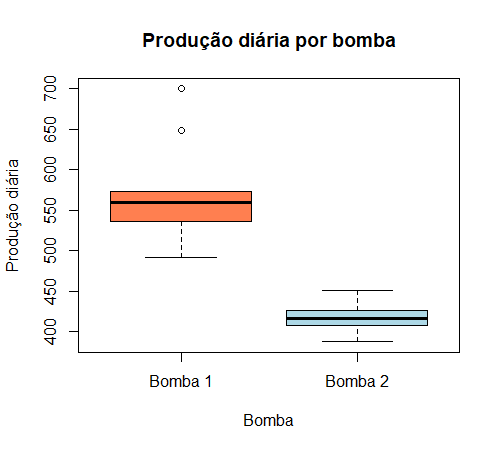
\includegraphics[width=9cm]{images/pumps/boxplotRandomSample.png}}
    \caption{Box plot of the daily production from pumps 1 and 2 on the days of the random sample.}
    \label{pump_boxplot_randomSample}
\end{figure}

Analyzing the results obtained, we observe that pump 1 has a higher daily production of barrels of oil than pump 2.

It can also be observed that bomb 2 has a more symmetrical distribution compared to bomb 1 since its median is practically centralized and the minimum and maximum values are not too far apart.

On the other hand, pump 1 has a more dispersed distribution, with the median displaced from the center and two upper outliers, without a defined maximum limit.\\

The fourth paragraph consisted of using the random sample from the previous paragraph to carry out a hypothesis test to verify whether the average daily oil production of pump 1 was higher than that of pump 2 in a period from June 1, 2013, to May 31, 2014.

To perform this comparison, the Student's t-test is the most appropriate since the samples are small (n = 10 < 30) and paired. In addition, it is possible to assume that the samples have a normal distribution since the box plot analysis suggests that the distributions of the daily productions of the two pumps are approximately symmetrical and without significant outliers.

So, two hypotheses were synthesized:

\begin{itemize}
    \item H0: The average daily oil production of pump 1 was less than or equal to the average daily oil production of pump 2;
    \item H1: The average daily oil production of pump 1 was higher than the average daily oil production of pump 2.
\end{itemize}

After performing the Student's t-test, we obtained a p-value of 2.175e-05.
Considering the standard significance level (5\%), we found that the p-value is less than alpha (0.05), so we can reject H0.
Thus, we conclude that there is statistical evidence to affirm that the average daily oil production of pump 1 is greater than that of pump 2 in the period from June 1, 2013, to May 31, 2014, with a 5\% significance.\\

The fifth and last subparagraph consisted of confirming whether the decision obtained in the test carried out in the previous paragraph corresponds to "reality".

To do so, first, we calculated the daily average of each pump using the data from the previous table, which contained the daily production averages of pumps 1 and 2. Then, we performed the difference between the values of the averages (in this case, we calculated the average of pump 1 minus the average of pump 2).

As the result of the difference was positive, we can conclude that the average daily oil production of pump 1 is greater than that of pump 2, thus confirming the decision obtained in the Student's t-test.

\subsection{Machine Learning Algorithms - Data Treatment}
The "Dados2.csv" dataset contains data about the precision of multiple machine learning algorithms , such as Support Vector Machines (SVM), Decision Tree (DT), K-nearest neighbors (KN), Radio Frequency (RF), Multilayer Perceptron (ML) and Gradient boosting (GB).
Through exploratory analysis, given more context, it is possible to find hidden to the naked eye information, allowing a deeper understanding of a certain context. For example the interconnection (correlation) between algorithms.

\section{Exploratory Analysis - Machine Learning Algorithms}
Since the exercise requests to examine the correlation between the accuracy of each pair of algorithms, it is necessary to, first, analyze the correlation between all algorithms. To achieve this it is necessary to make a correlation matrix between pairs of algorithms. When we make this matrix it is possible to affirm a lot of information from the results.

\begin{figure}[htbp]
    \centering{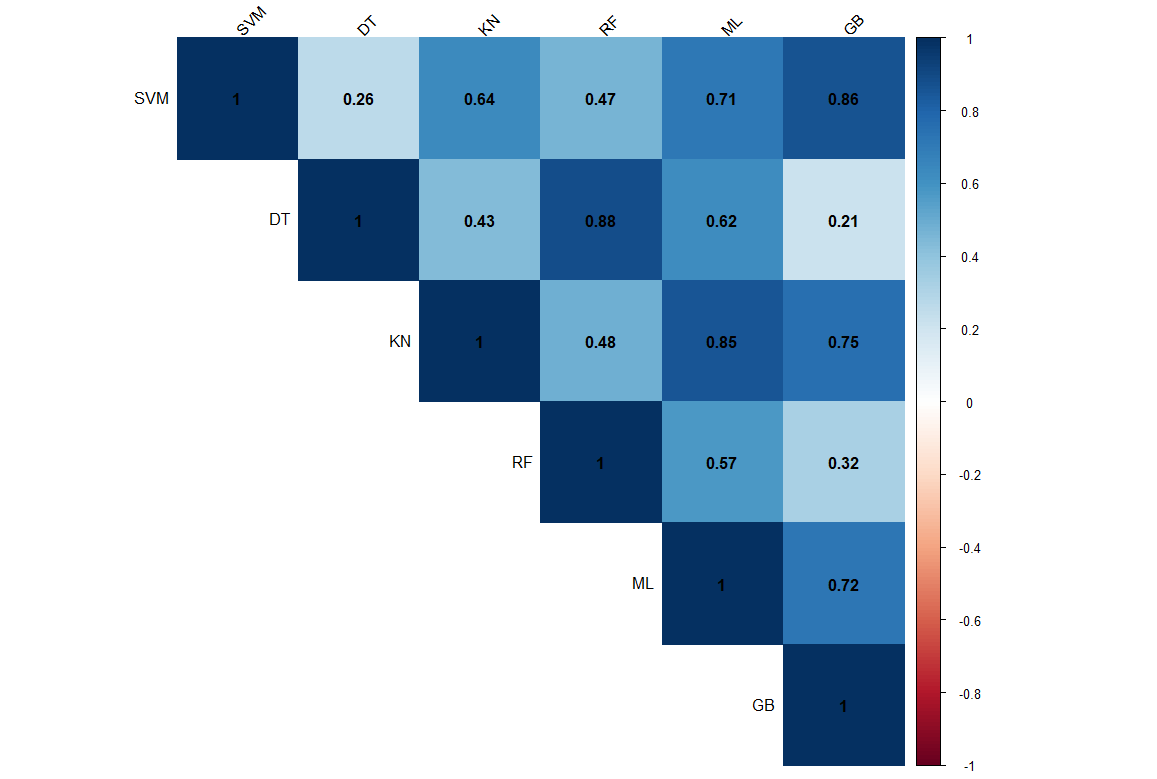
\includegraphics[width=9cm]{images/ex2/Matriz_Correlaçoes.png}}
    \caption{Corrplot of the correlation matrix.}
    \label{vehicle_boxplot}
\end{figure}

The correlation matrix presented depicts the inter correlation among the accuracy of the six distinct machine learning algorithms explained before. The values within the matrix range from -1 to 1, where 1 signifies a perfect positive correlation, 0 represents no correlation, and -1 indicates a perfect negative correlation.

The following observations can be obtained:

\begin{itemize}
    \item The main diagonal, which reveals the correlation between the same machine learning technique, consistently exhibits a value of 1, as the correlation between the accuracy of a technique and itself is perfectly positive;
    \item A strong positive correlation (0.86) is observed between SVM and GB, implying that these techniques are related and may perform well in comparable tasks;
    \item DT exhibits a strong positive correlation (0.88) with RF, suggesting that these two techniques are related and may perform well in comparable tasks;
    \item KN and ML exhibit a strong positive correlation (0.85), indicating that these two techniques are related and may perform well in comparable tasks;
    \item The correlation between SVM and KN is moderate (0.64), which suggests that these techniques may also be related, but not as strongly as SVM and GB, or DT and RF;
    \item DT exhibits a moderate correlation (0.62) with ML, while GB shows a moderate correlation (0.72) with ML. This finding implies that these techniques may also be related, albeit not as strongly as DT and RF, or SVM and GB;
    \item There is a weak positive correlation (0.21) between DT and GB, suggesting that these two techniques may have some degree of similarity, but are not strongly related. The same goes between SVM and DT; RF and GB;
    \item No negative correlations are evident from the presented matrix, as all values range between 0 and 1, with 1 indicating perfect positive correlation and 0 indicating no correlation.
\end{itemize}

In summary, the correlation matrix presented highlights the varying intercorrelations between machine learning techniques concerning accuracy. This information can be leveraged to choose the most suitable machine learning technique for a specific task.

The second exercise requests to perform a hypothesis test to see if there are significant differences between the precision of different algorithms. To achieve that we must follow some rigorous steps to affirm if we can perform parametric tests or non-parametric tests.

To make statements about a particular population of data, we resort to parametric tests. To do so, we must follow the following steps:

First, we formulate our test hypotheses:

\begin{itemize}
    \item H0: There are significant differences between the precision of different algorithms;
    \item H1: There are no significant differences between the precision of different algorithms.\\
\end{itemize}

Second, is the dependent variable (precision) continuous? Yes it is a continuous variable. \\

Third, does the independent variable (algorithms) have two or more algorithm groups? Yes, there are six algorithms. \\

Fourth, are the observations dependent since, according to the precision of the algorithms, some are interconnected with others, as can be observed through the correlation matrix in exercise one, which shows indices of interconnection among several algorithms? This may explain the interdependence in the samples. \\

Fifth, do the observations have significant outliers? To assess this, we created a boxplot to verify if there are any outliers outside the whiskers.

\begin{figure}[H]
    \centering{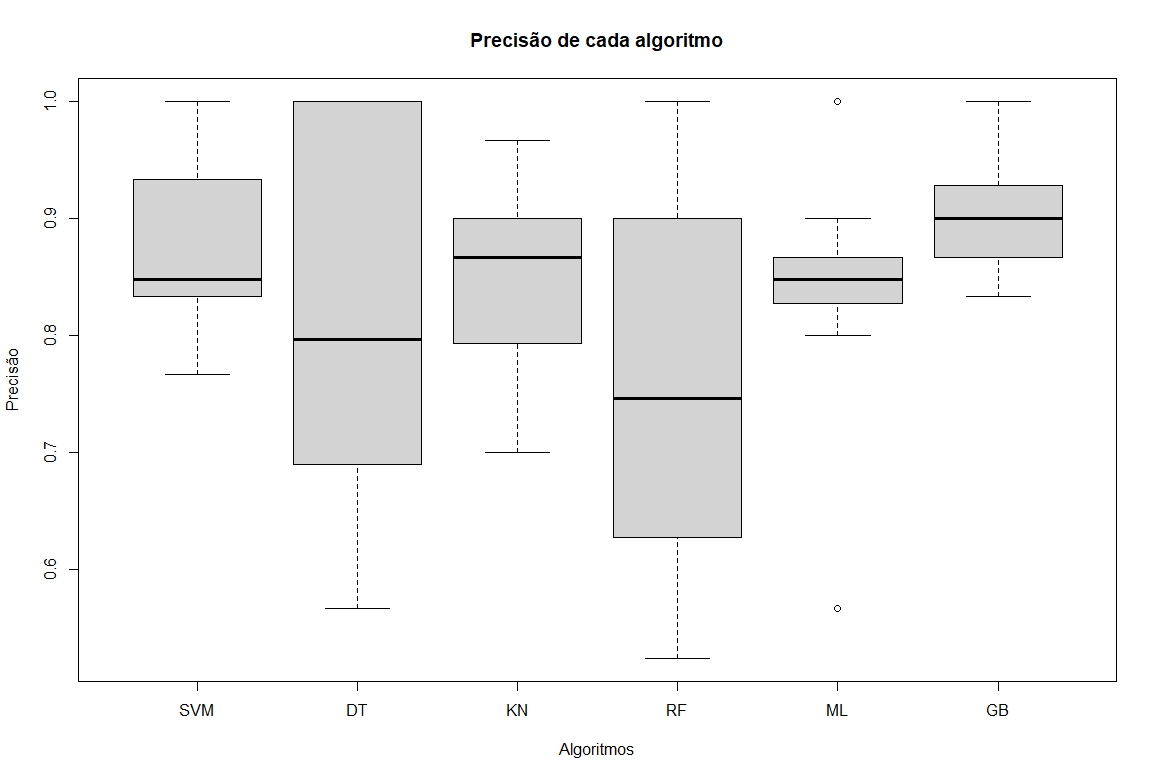
\includegraphics[width=9cm]{images/ex2/BoxPlot_Precisao.png}}
    \caption{Boxplot of the precision values according to the algorithms.}
    \label{vehicle_boxplot}
\end{figure}

Analyzing the results obtained, we observe that the precision of some algorithms differs drastically from others. This can be observed in the boxplot.

As we can see, some algorithms disperse (in this case have a more variety of values) such as DF and RF, while ML and GB have a smaller group of values.

The median (represented by the darker line inside the boxes) of the  ML and GB algorithms are the more symmetrical ones, while DT and RF are more non-symmetrical.

Another relevant factor to highlight is the distance between the minimum and maximum values of each algorithm, which indicates the data dispersion. In DT and RF algorithms, there is a large spread of data, while in ML and GB algorithms, the spread is smaller.

Furthermore, the box (interquartile range - IQR) of the RF algorithm is larger than any other algorithm, which indicates a higher frequency in the data distribution.

After analyzing the boxplot, it was possible to confirm that significant outliers do indeed exist, as precision is a continuous variable obtained from a measurement. 

Sixth, although we had a clear view that significant outliers existed, a Shapiro test, which verifies if a dependent variable is normally distributed was performed for each algorithm.

For the KN, GB, RF, SVM, and DT algorithms, the obtained significance level was 0.6926, 0.5125, 0.3138, 0.2687, and 0.06772 which could lead us to believe that homogeneity was achieved.

However, for the ML algorithm, the significance level was 0.02138, which is inferior to the necessary 0.05, which obligates us to refute the theory which implies that the dependent variable is normally distributed.

We could also use histograms to verify if the dependent variable is normally distributed. Since we already concluded that the ML algorithm is not, we will only show this Histogram algorithm.

\begin{figure}[H]
    \centering{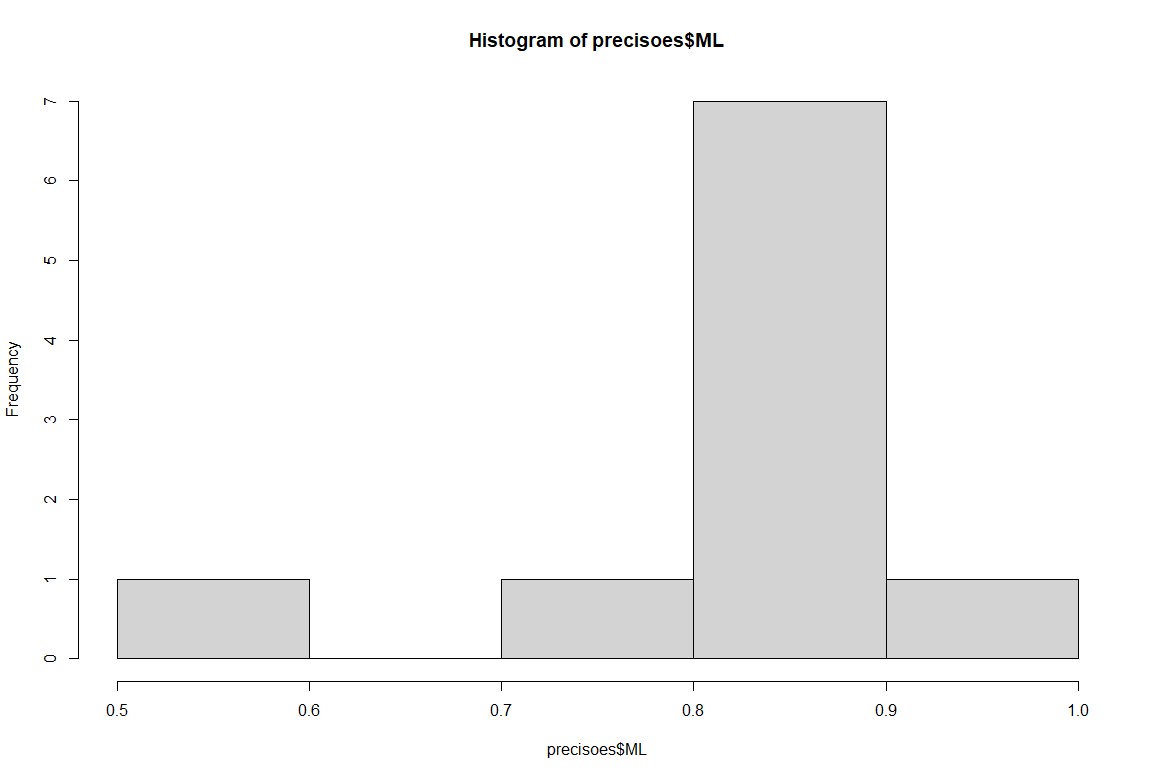
\includegraphics[width=9cm]{images/ex2/ML_Histrogram.png}}
    \caption{Boxplot of the precision values of the ML algorithm.}
    \label{vehicle_boxplot}
\end{figure}

With this conclusion taken, the possibility to use a parametric test such as One-Way ANOVA is ended. So, to test our original theory, we must use a non-parametric test. And, for that purpose, we reached the possibility of a Friedman test.

In order to verify which of the hypotheses is correct, it will be necessary to use a Friedman test, since the samples are interrelated. Kruskal-Wallis could be a valid option if the data were independent from each other. However, as we saw from section a) and the explanation of the variables, we cannot conclude that the data is independent.

The Friedman test measures data on an ordinal scale and the samples are related. In our case, this situation is verified and confirmed. Therefore, we will apply a study based on a Friedman test.

After making the Friedman test we obtain a p-value of 0.1212 which is superior than the significance level so we can't reject H0. There is no statistical evidence to claim that there are significant differences between the precision of the different algorithms.

In the last exercise it was requested to make post-hoc study in case there were significant differences between the precision of the different algorithms, but, as we seen in the previous exercise there is no significant differences, so there is no need to make that type of study.

\subsection{Vehicles Data set - Data Treatment}
The "DADOS3.csv" data set contains data about vehicle characteristics, such as acceleration, the number of cylinders in the engine, along with horsepower and the vehicle's weight.
Through exploratory analysis, given more context, it is possible to find hidden to the naked eye information, allowing a deeper understanding of a certain context.
For instance, a brand or a specific model.
\section{Exploratory Analysis - Vehicles}
Since the exercise requests to examine if there are significant differences in acceleration values between the three engine cylinder groups, 
it is pivotal to partition the acceleration values according to the number of cylinders. 
This is required because the proposed challenge questions if there are significant differences in the acceleration between vehicles, 
which leads to a concrete hypothesis test, allowing us to answer this question through the provided accelerations per cylinder.
So, two hypotheses were synthesized:

\begin{itemize}
    \item H0: There aren't significant differences between acceleration values according to the cylinder count;
    \item H1: There are significant differences between acceleration values between the distinct groups.
\end{itemize}

After formulating the two possible premises, we observe that the faced test is bilateral.
This is due to us facing an interest in solely finding out whether the mean acceleration of one group is higher or lower than the other one.\\

To prepare the data for the performed analysis, we first imported the data set, which then was segregated into three distinct categories.
These are the different numbers of cylinder counts: 4, 6 and 8.\\

After setting up the required data, for the trial to be started, we needed to evaluate which kind of test could be performed on this population.
Starting with ANOVA, there are 6 exclusive steps which need to be accomplished.\\

First, is the dependent variable continuous? Because it varies according to the number of cylinders and takes infinite possibilities of values within a certain range, it is considered so.

Second, the independent variable (number of cylinders) has 3 groups of values, which complies with the two or plus variable groups.

Third, the observations are independent, considering that according to the essay, the number of cylinders is the key factor to consider in this variation.

Fourth, do the observations have significant outliers? To answer this question, a box plot, which is a type of graphic that displays the median, quartiles, and outliers of the data was engendered.

\begin{figure}[htbp]
    \centering{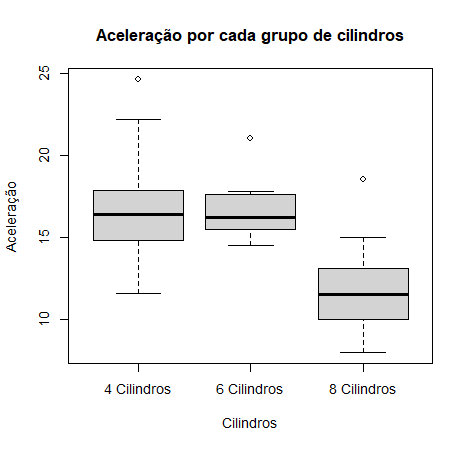
\includegraphics[width=9cm]{images/vehicles/boxplot.png}}
    \caption{Box plot of the acceleration values according to the number of cylinders.}
    \label{vehicle_boxplot}
\end{figure}

At first sight, the results demonstrate that the 4-cylinder group has the highest median acceleration value (16.4), closely followed by the 6-cylinder group (16.2), 
which pulls a significant distance from the 8-cylinder engines acceleration (11.5). 
The interquartile range on 4 and 8-cylinders is much ampler than the 6-cylinders.
Its whiskers are also much more wide-ranging. 
Diving deeper into the quartiles analysis, for 4-cylinder powered vehicles, the quartile inferior limit is 10.2, with its superior limit around 22.4, close to the represented outlier. 
For the 6-cylinder, the inferior and superior limits were 12.3 and 20.8, respectively.
Lastly, on the 8-cylinder designed cars, 5.35 and 17.8.

After closely observing the box plot it is confirmed that significant outliers exist, considering that acceleration is a continuous variable.
These are random points outside of the whiskers(highest and lowest observations within 1.5 times the interquartile range), particularly important when applied to a real-life scenario.
These could be explained by a vast number of variables, for instance, tyre pressure, which is outside of our scope.
Outliers are one of the most interesting/curious parts of a box plot since they can reveal hidden causes.\\

However, 6-cylinder cars produce much more consistent results, while the remaining two have a wider spectre of traduced power.

Fifth, although we had a clear view that significant outliers existed, a Shapiro test, which verifies if a dependent variable is normally distributed was performed for each cylinder group.
For the 4-cylinder and 8-cylinder groups, the obtained significance level was 0.1056 and 0.2729, which could lead us to believe that homogeneity was achieved.
However, for the 6-cylinder group, the significance level peaked at 0.03628, which is inferior to the necessary 0.05, 
which obligates us to refute the theory which implies that the dependent variable is normally distributed.

With this conclusion taken, the possibility to use a parametric test such as One-Way ANOVA is ended. So, to test our original theory, we must use a 
non-parametric test. And, for that purpose, we reached the Kruskal-Wallis test.

On a Kruskal-Wallis test, if the predetermined significance level (which in this case is 0.05) is not met, the null hypothesis is rejected.
So, after fulfilling it, we could reach the conclusion that our p-value is 2.795e-11, leading to rejection H0, meaning that H1 is the accepted hypothesis, 
stating that there are significant differences between the cylinder groups.

\section{Linear Regression}

Linear regression is frequently used to forecast and analyze correlations between variables. On a practical side, it is commonly adopted in fields such as economics or engineering.
During the analysis of the data set, four different plots were generated, which allowed us to verify the differences between the measured accelerations and the expected ones by the model.
The residuals sat around a median of -0.2788.

\subsection{Residuals vs Leverage}

The Residuals vs Leverage plot allows an analyst to verify if the provided data set has many outliers which give insights to the researchers if they are being misled.
In this particular case, it shows a big concentration of data around the [-2,2] Residuals mark, 
with only a minority on other parts of the plot, which leads us to believe that the outliers are not influential on the interpreted result.

\begin{figure}[H]
    \centering{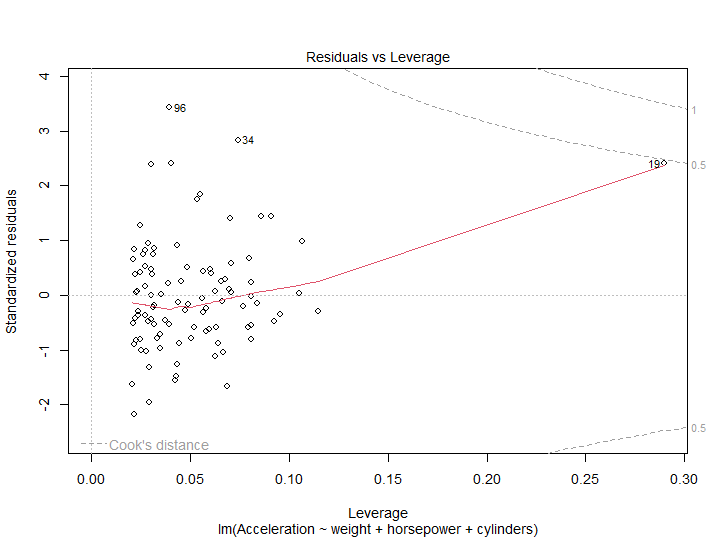
\includegraphics[width=9cm]{images/vehicles/residualsLeverage.png}}
    \caption{Graphic of the Residuals vs Leverage Regression Model}
    \label{residualsLeverage}
\end{figure}

\subsection{Residuals vs Fitted}

The Residuals vs Fitted plot allows an investigator to evaluate the provided data's quality and even possibly detect hidden patterns.
If the plot is properly adjusted between the two available variables, all the marked spots should be around 0. Analysing the given plot, even though the flagged values are around the 0 mark, 
we can observe a function slightly shaped like a very wide V, which makes us conclude that there may be some residue on certain groups, with the values being under/overestimated.
Ideally, the function should be as straight as possible, with the values spread around.

\begin{figure}[H]
    \centering{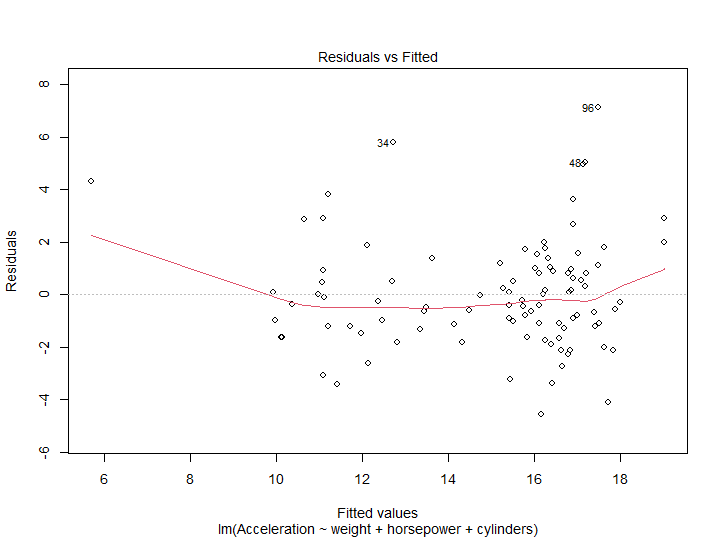
\includegraphics[width=9cm]{images/vehicles/residualsFitted.png}}
    \caption{Graphic of the Residuals vs Fitted Linear Regression Model}
    \label{residualsFitted}
\end{figure}

\subsection{Scale vs Location}

The Scale vs Location plot is another type of residual graphic used on linear regression.
Since this type of plot shows represents the square root of each value, for a graphic to be valuable (homoscedasticity), 
the points on the plot must be scattered horizontally around the line, which is the current case.

\begin{figure}[H]
    \centering{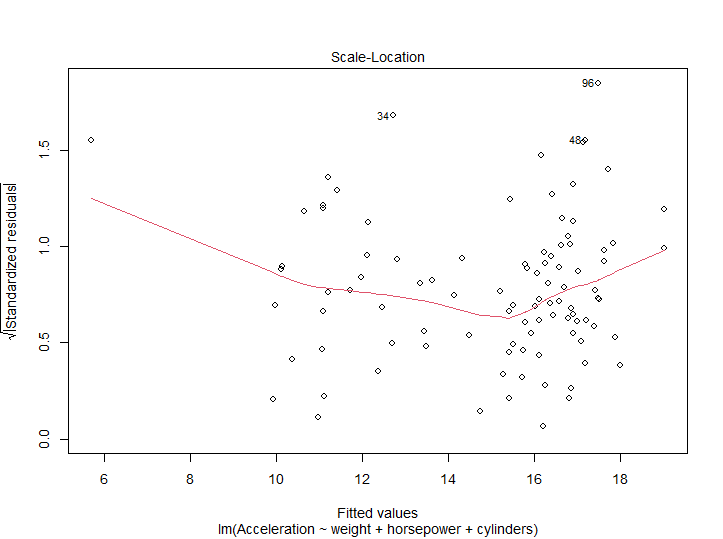
\includegraphics[width=9cm]{images/vehicles/scaleLocation.png}}
    \caption{Graphic of the Scale-Location Linear Regression Model}
    \label{scaleLocation}
\end{figure}

\subsection{Normal Q-Q}

Lastly, the Normal Q-Q Linear Regression plot allowed us to assess if the data set was normally distributed.
Ideally, we want the points to be distributed closer to the line, which means that they would be normally distributed. 
Upon analysis, they are falling on an almost straight line, opposite to a bowed or S-pattern (which would represent skewness), this one is almost perfectly shaped, 
with a reduced number of outliers present.

\begin{figure}[H]
    \centering{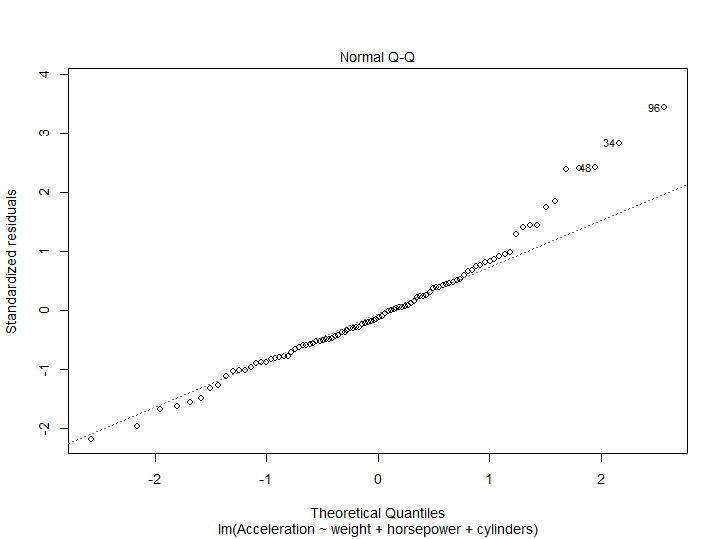
\includegraphics[width=9cm]{images/vehicles/normalQQ.png}}
    \caption{Graphic of the Normal Q-Q Linear Regression Model}
    \label{normalQQ}
\end{figure}

The positive feedback from the given plots allowed us to conclude that the data set is certainly to be trustworthy.

\section{Prediction}

For the last exercise, it was requested to predict what would the acceleration of a car be if the engine had 4 cylinders, weighed 2950 kg and it had 100 horsepower. 
After performing a prediction, an acceleration value of 17.308, which belongs to 15\% 
between the 50\% below 16.4 and 75\% 17.85 is fitting into the provided graphics.

\section{Conclusion}

For the first exercise, we had to import the data from the data set provided to compare the three pumps.
After including a new column with the representation of time in the POSIXct format, we were able to carry out the necessary analyses to meet the proposed objectives. For this, we built several graphs to compare the engine temperature and the daily production of barrels of oil from the three pumps in a specific time interval. The latter whose dates were obtained through a random sample.
In addition, a hypothesis test was performed to compare the average daily oil production of two pumps.\\

For the second exercise, we had to extract the data from the dataset to compare all algorithms. Firstly we did a correlation matrix to determine which algorithms had a stronger relationship between them. Then we had to make a test to study if there were significant differences between the precision of all algorithms in which we concluded, based on a Friedman test, that there was no statistical evidence that could prove this hypothesis. In the last exercise, since we proved that there were no significant differences between the algorithms we can not make a post-hoc study to the test previously performed. \\

For the third exercise, to put it concisely, the conclusion we extracted from the data set is that when comparing the 3 groups, vehicles which have 4 cylinders have the higher acceleration, 
closely followed by 6 cylinders, with 8 cylinders vehicles bottoming out the list with the least acceleration.

\begin{thebibliography}{00}
\bibitem{b1} How to Use Q-Q Plots to Check Normality - Statology. (n.d.). Retrieved April 13, 2023, from \url{https://www.statology.org/q-q-plot-normality/}
\bibitem{b2} What is Considered a Good vs. Bad Residual Plot? - Statology. (n.d.). Retrieved April 13, 2023, from \url{https://www.statology.org/good-vs-bad-residual-plot/}
\bibitem{b3} How to Interpret a Scale-Location Plot (With Examples). (n.d.). Retrieved April 13, 2023, from \url{https://www.statology.org/scale-location-plot/}
\bibitem{b4} What is a Residuals vs. Leverage Plot? (Definition \& Example) - Statology. (n.d.). Retrieved April 13, 2023, from \url{"https://www.statology.org/residuals-vs-leverage-plot/}
\bibitem{b5} O que são amostras independentes? - Minitab. (n.d.). Retrieved April 13, 2023, from \url{https://support.minitab.com/pt-br/minitab/20/help-and-how-to/statistics/basic-statistics/supporting-topics/tests-of-means/what-are-independent-samples/}
\bibitem{b6} How to perform the Kruskal-Wallis test in R? | R-bloggers. Retrieved April 12, 2023, from \url{https://www.r-bloggers.com/2022/05/how-to-perform-the-kruskal-wallis-test-in-r/}
\bibitem{b7} A Complete Guide to Box Plots | Tutorial by Chartio. Retrieved April 12, 2023, from \url{https://chartio.com/learn/charts/box-plot-complete-guide/}
\end{thebibliography}
\vspace{12pt}

\end{document}
